\documentclass[conference]{IEEEtran}

\usepackage{cite}
\usepackage{amsmath,amssymb,amsfonts}
\usepackage{algorithmic}
\usepackage{graphicx}
\usepackage{textcomp}
\usepackage{xcolor}
\usepackage{hyperref}
\usepackage{subcaption}

\graphicspath{{figures/}}
\hypersetup{hidelinks}

\begin{document}
\bibliographystyle{IEEEtran}

\title{Breast Cancer Detection in Histopathology Images using Ensemble Balancing\\
  {\footnotesize Course project for ECE9603 Introduction to Data Analytics}
}

\author{
  \IEEEauthorblockN{Abubaker Hameda}
  \IEEEauthorblockA{\textit{Electrical and Computer Engineering} \\
    \textit{(University of Western Ontario)} \\
London, Canada \\
ahameda4@uwo.ca}
\and
  \IEEEauthorblockN{Aisha Edrah}
  \IEEEauthorblockA{\textit{Electrical and Computer Engineering} \\
    \textit{(University of Western Ontario)} \\
London, Canada \\
aedrah@uwo.ca}
\and
  \IEEEauthorblockN{Muhammad Khan}
  \IEEEauthorblockA{\textit{Electrical and Computer Engineering} \\
    \textit{(University of Western Ontario)} \\
London, Canada \\
mkha83@uwo.ca}
\and
  \IEEEauthorblockN{Patrick Egan}
  \IEEEauthorblockA{\textit{Electrical and Computer Engineering} \\
    \textit{(University of Western Ontario)} \\
London, Canada \\
pegan3@uwo.ca}
\and
  \IEEEauthorblockN{Spencer Vecile}
  \IEEEauthorblockA{\textit{Electrical and Computer Engineering} \\
    \textit{(University of Western Ontario)} \\
London, Canada \\
svecile@uwo.ca}
}

\maketitle

\begin{abstract}
  Breast cancer is a looming healthcare concern which is costing many female
  deaths around the world each year. Early disease detection can therefore play
  a vital role in saving human lives as well as reducing healthcare costs.
  Recent advances in Machine Learning have paved the way for detection of cancer
  through early stages. All machine learning techniques use for classification
  are based upon the assumption that various classes are near equal number of
  samples in the entire dataset. When this assumption is no true, researchers
  must develop a technique to achieve this balance during the pre-processing
  phase. In this paper we present our technique of using ensemble learning for
  the purpose of achieving class balance.
\end{abstract}

\begin{IEEEkeywords}
  Breast Cancer Detection, Ensemble Learning, Histopathology Images,
  Neural Networks, Class Imbalance
\end{IEEEkeywords}

\section{Introduction}
\subsection{Problem Definition}
Breast cancer is the most common form of cancer in women [1]. It is estimated
by the American Cancer Society that in 2021, 281550 new cases will be diagnosed
with estimated 43600 deaths [2]. Histopathology is the study of tissue cells
at microscopic level with the objective to identify the changes occurring in
cells due to a particular disease. For diagnosing cancerous cells and
identifying stages of cancer progression, histopathology has been used in
numerous studies. [], [], [] are just a few examples to mention. Recent
advances in machine learning, in particular, application of neural networks
for image classification, have fuelled diagnostic image processing as well as
histopathology research. Identifying the type of breast cancer is a significant
step towards receiving treatment. Automating this process can help accelerate
the diagnosis and minimize the chances of human error as well as reduce the
risk of misdiagnosing the stage of breast cancer. If  cancer is detected in
early stages, the survival rate can reach 80\% [3]. Invasive Ductal Carcinoma
or IDC is the most common form of breast cancer, making up about 80\% of all
breast cancer cases [4]. By utilizing available scanned images of IDC cases,
the automation can be partially achieved. At the very least, it can assist in
preventing a potential misdiagnosis in a patient who may have one of the more
rare and serious forms of breast cancer.
\subsection{Motivation}
This project is aimed at binary classification of breast cancer histopathology
images. The selected dataset contains samples from multiple patients as well as
multiple samples from the same patient and is large enough to extract good
quality images. This provided interesting opportunities to improve diagnostic
accuracy in pre-processing as well as model building and training phases, all
the while allowing us to evaluate different neural network architectures and
do comparative study of results. Standard metrics have been used to measure the
performance in each case and a detailed discussion is presented.
\\ \indent The rest of this paper is organized as follows: Section II presents
background. Section III outlines the related work. Section IV describes the
methodology/process. Section V illustrates the result and is followed by
conclusions in the last section.

\section{Background}
Machine Learning is the automated process in which a computer program reads
data and finds patterns of interests [5]. Classification is the machine learning
process whereby data is classified into two or more classes. Supervised rest
classification is the process where the input data contains labels for the
class of each data record. A machine learning algorithm learns the relationship
of the labels with the of the fields of the data records in a process called
training. By learning the patterns and relationship the learned algorithm can
then classify new, never-encountered, data records with one of the labels for
the classes [6].
\\ \indent A Neural Network is a special type of machine learning structure
that can find complex non-linear relationships and patterns in data. Neural
Network’s structure resembles, albeit very simplified, the way natural neural
brains are structured. Neural Networks are composed of neurons, where each
neuron has multiple input and a single output. Neurons are structured in layers
where the first layer corresponds to the input of each data value in the data
record and output is a real number between 0 and 1. The output layer corresponds
to a single neuron for two classes or n neurons for n classes. Then there are
hidden layers between input and output layers where each hidden layer is
composed of several neurons. The number of hidden layers and the number of
neurons each layer contains depends on the problem and is part of the design of
the architecture of the neural network. All layers are combinatorially connected
with the neurons in the adjacent layer [7].

\section{Related Work}
There has been a wealth of research in applications of Machine Learning to
diagnose the presence or absence of cancer in histopathology images as well as
in grading and sub-typing of the tumor tissue.
\\ \indent BACH database [8] was specifically created containing annotated
images to challenge and evaluate various classification algorithms. The winning
algorithm for this challenge was based on the Convolutional Neural Network. The
most accuracy achieved was 87\%.
\\ \indent Hierarchical classification of breast cancer [9] was carried out on
the Convolutional Neural Network. They also classified the stages of the
detected cancer. Alom et. al. also performed classification of breast cancer
using deep neural networks [10]  80- 85\% accuracy was achieved by yet another
attempt to classify breast cancer [11]. Another attempt [12] reported 91.5\%
accuracy on BreakHis dataset. Another team [13]. Reported 94\% to 100\% accuracy
on a small dataset.
\\ \indent Other approaches such as cubic SVM [14] achieved 92.3\% accuracy.
\\ \indent Class imbalance problem, i.e., when in supervised classification
tasks some labeled class(es) have significantly larger number examples that
other class(es) in the training set, is a problem that is create significant
accuracy issues due to bias classifications solutions. It is especially
pertinent in classifying cancer as almost all image datasets contain far too
many examples for benign tumors vs examples with cancerous tumors.  For a
detailed study on class imbalance problems in neural networks see Buda et al
[15] , which shows that even modest imbalance creates substantial deterioration
of classifier performance. [16] discuss class imbalance problems being
especially significant in the medical domain.
\\ \indent One solution among others in handling class imbalance problems is
weighted loss function [17] . For example, batch-weighted loss function was
successfully used for more accurate heartbeat classification [18].
\\ \indent Another approach is using over or under sampling; where under
sampling is shown more promising that oversampling, see [19]  and  [20].

\section{Dataset}
For the purpose of this project, an openly available dataset was obtained from
Kaggle  The dataset for this project is a pre-processed version of another
dataset. The original dataset contained 279 whole slide mount images of breast
cancer specimens scanned at 40x. Then from each whole slide mount image
sections of 50 x 50 pixels were taken which either contained benign or
malignant cells. In total, 277,524 color sections of size 50 x 50 were
extracted from all the slide images, which breaks down into 198,738 Invasive
Ductal Carcinoma (IDC) negative (class 0) and 78,786 IDC positive (class 1).
Each patient has their own file which breaks down into two more folders, one
for positive class and one for negative class. The number of images in each
of the classes for a specific patient is random. Each image is labeled with
the format u\_xX\_yY\_classC.png where u is patient ID, x is the x coordinate
where the 50 x 50 section was taken from the original whole slide image, y
is the y coordinate where the section was taken from the original image and
then C is the class which is either 0 or 1. The dataset is not separated into
train, validation and test sets yet so that will have to be done based on
patient ID so leakage between the sets is not introduced. The original dataset
the sections were taken from is not available.

\section{Methodology}
\subsection{Base Model}
The base model was Google’s pre-trained EfficientnetB0 (EN) with a modified
classification layer. The pretrained EN was trained on ImageNet and used as a
feature extractor. Due to it only being needed as a feature extractor its model
parameters were frozen and set as not trainable to speed up the training
process. The last classification layer of EN was removed and replaced with a
trainable classification model consisting of 3 fully connected linear layers,
dropout, batchnorm1d and ReLU. These layers Shrink the features from 1280 at
the output of EN to one which is out binary output which can be seen in Fig~\ref{base_model}.

\begin{figure}[tp]
  \centering
  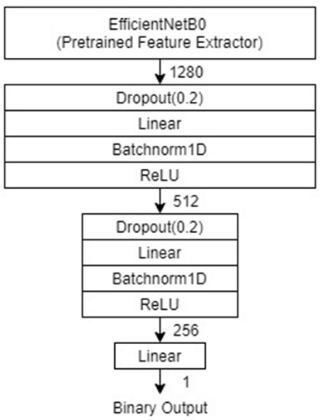
\includegraphics[scale=0.3]{base_model.png}
  \caption{Base model using Google's Efficientnet B0 with a classification
    layer replacing the output layer}
  \label{base_model}
\end{figure}

This model is what we use to compare our method of dataset balancing to more
traditional methods and is also the main building block of our ensemble
balancing method.

\subsection{Ensemble Balancing}
\label{section:ensemble_balancing}
The method presented in this paper is a novel approach to dealing with large
class imbalance in medical image datasets. Balancing of the training set is the
focus as the validation and testing sets should be an accurate representation
of the real world, including imbalances. To start the number of samples in the
overrepresented class is divided by the number of samples in the
underrepresented class to determine the number of models and chunks needed.
The larger class is then split into chunks of equal size to match the size of
the smaller class. Each of the larger class’s chunks are concatenated with a
copy of the smaller class to make up several balanced, equal sized training
sets. Each of these training sets are given a copy of the base model shown in
Fig~\ref{base_model} and trained individually. When making predictions on the test set
each of the models are fed the samples and the output from all the models is
averaged and becomes the prediction for that sample.  An example of this
Process can be seen in Fig~\ref{ensemble_model}. This method should eliminate the
overfitting caused by oversampling the minority class since each model only
sees each of the minority class samples once. It should also eliminate the
wasting of data caused by under-sampling the majority class since all the
samples are still used; each of the models just sees a different part of the
majority class. Then the model’s predictions are averaged so they form one
whole model that has seen the entire dataset.
\begin{figure}[bp]
  \centering
  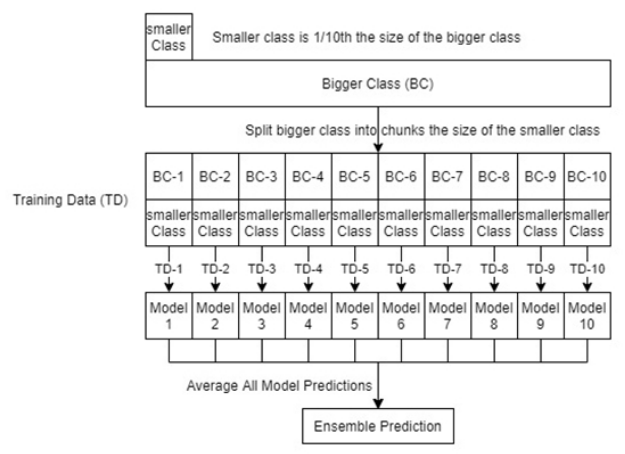
\includegraphics[scale=0.3]{ensemble_model.png}
  \caption{Ensemble model which uses a group of clasiffiers at the output of
    the Google Efficientnet model to collectively determine the output class}
  \label{ensemble_model}
\end{figure}

\section{Evaluation}
\subsection{Preprocessing}
Pytorch data loaders were used to load the data into the model in batches of
size 128. Before the model sees the image, the data loader will resize the
images to 224x224 to fit into EfficientnetB0. It will then randomly flip the
image in the vertical and horizontal direction to reduce overfitting. Lastly
it will normalize the image using [0.485, 0.456, 0.406] for the mean in the
RBG layers and, [0.229, 0.224, 0.225] for the standard deviation in the RBG
layers as is required for EfficientnetB0.

\subsection{Base Model}
\subsubsection{Dataset}
Two versions of the dataset were used for evaluation. The first was the
original dataset and the second was the original dataset but the smaller class
was randomly sampled to make it 1/10th the size of the majority class. This was
done to make the dataset imbalance more apparent since the original dataset was
72\% cancer negative and 28\% cancer positive which isn’t that big of a class
imbalance.
\subsubsection{Model Training}
weighted loss functions including: Dice Loss, Binary Cross Entropy Dice Loss,
JaccardIoU Loss, Focal Loss, Tversky Loss, Focal Tversky Loss and Weighted
Binary Cross Entropy. The training would run for a maximum of 10 epochs with
early stopping being set to stop training if there were 2 epochs without
improvement in the validation loss. The learning rate was 0.001 and Adam’s
optimization was used with default parameters.

\subsection{Ensemble Model}
\subsubsection{Dataset}
To make comparison possible the same two datasets that were used in the base
model were used in the ensemble model. For the original dataset the negative
class was split into 3 equal sized pieces and the positive class was copied and
concatenated to each of them. This created 3 different training sets of equal
size containing 47\% negative samples and 53\% positive samples. This can be seen
in Fig~\ref{ensemble_data_split}.
\begin{figure}[bp]
  \centering
  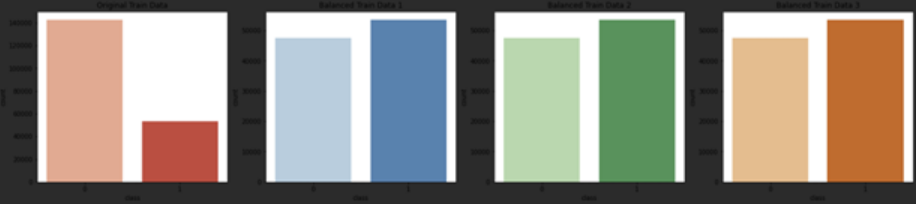
\includegraphics[scale=0.2]{ensemble_data_split.png}
  \caption{Ensemble model training data.  Before split (red) and after split
    (blue, green and orange)}
  \label{ensemble_data_split}
\end{figure}
The second dataset was split in the same way except the negative class was
split into 10 pieces, making 10 training sets each with a perfect 50\% positive
samples and 50\% negative samples.
\subsubsection{Model Training}
Each of the models that made up the ensemble would be trained individually and
with the same hyperparameters as the base model except the loss function. The
loss function for each of the models in the ensemble was binary cross entropy.

\subsection{Weighted Loss Functions}
For comparison against the ensemble model presented in this paper, weighted
loss functions were applied to the base model.  This model, like the proposed
model, used the Google EfficientNet B0 as a base for feature extraction coupled
with a single simple classification model with the same structure as the
proposed model.  The primary difference being that several different loss
functions with special weights were applied to this simplified model to see how
this simpler model would perform on the same dataset.  The weights used were
calculated based on the proportion of positive to negative classes.
\\ \indent As a weightless simple point of reference, an unweighted loss
function known as the “Dice Loss” function was applied.  This loss function is
based off of the popular “Dice coefficient” used in computer vision
applications to calculate the similarity between images (Dice loss equation)
~\cite{loss_function_survey}.  Because this loss function was created with
image segmentation in mind, and the model was designed to segment input image
patches into positive or negative classes, it seemed like a good fit.  In
contrast to this unweighted function, the Binary Cross Entropy loss function
(also used in the ensemble model) was tested with class weights along with the
Tversky and Focal loss functions.  The Binary Cross Entropy, as provided
through the pytorch library, is a strong loss function for classification
models in general (BCE loss equation).  The class weights were applied to this
loss function by calculating a tensor with class weights in positions
corresponding with their associated samples so they could be applied before the
loss function combined the individual error of every sample.  The Tversky loss
function is a unique selection in that it calculates loss based on the amount
of true positives (TP), false positives (FP) and false negatives (FN) (Tversky
Loss Equation).  The class weights were applied as the “alpha” and “beta”
weights to adjust the significance of false positives and false negatives
respectively.  By making false negatives more heavy, this model provided a
“sensitivity” metric which could show how effective the model could be in
identifying positive cases of cancer.  The Focal loss function was designed
specifically for datasets with high class imbalance.  It addresses a class
imbalance by weighing “easy examples” with less significance and “harder
examples” with greater significance using the modulating factor gamma (Focal
Loss Equation) ~\cite{loss_function_survey}.  In this project an alpha of 0.8
and a modulating factor (gamma) of 2 were applied to the base model used for
comparison in the results section.  This seemed fairly applicable because each
patient had far more cancer-free image patches in their skin samples than
patches with cancer in them.  Because Focal loss uses the Binary Cross Entropy
loss function internally, the class weights were applied similarly to how they
were for the Binary Cross Entropy with Sigmoid layer (BCEWithLogits) loss
function.

\subsection{Testing}
To evaluate our model’s performance against the base models, a separate test
set was created that had a similar distribution to the original dataset, so no
balancing was done here. All the models were given the test set and performance
metrics were calculated including false positives, false negatives, true
positives, true negatives, balanced accuracy, specificity, sensitivity,
precision and AUROC score. The most important being the balanced accuracy and
sensitivity since this is a medical application false negatives are much worse
than false positives. However, in the case of imbalanced data where the
negative class is much larger, specificity should be taken lightly as the model
may just learn to predict always negative since that class is much larger.


\section{Results}
\subsection{Training Against Original Dataset}
In the first round of testing where each model was tested against the original
dataset with negative to positive class ratio 3:1, the ensemble model was
surprisingly outperformed.  Aside from the base model using binary cross
entropy, the base models and ensemble appear to have relatively similar
performance with respect to balanced accuracy as shown in Fig~\ref{original_data_balanced_accuracy}.
\begin{figure}[bp]
  \centering
  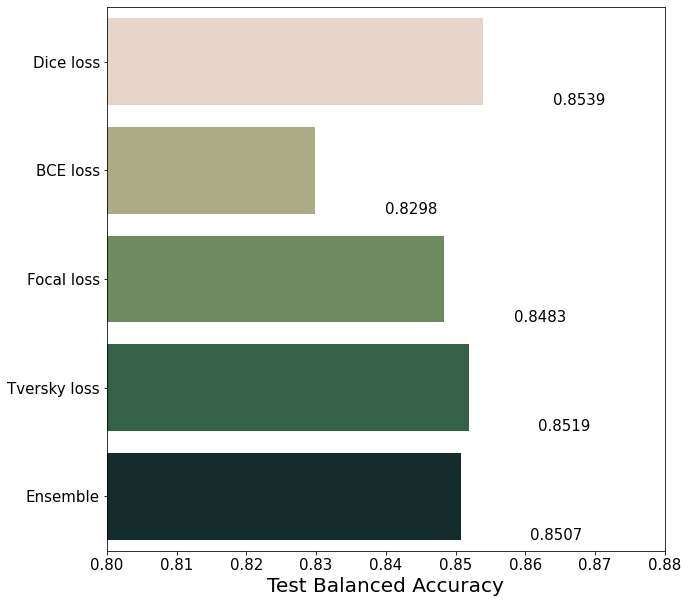
\includegraphics[scale=0.2]{original_data_balanced_accuracy.png}
  \caption{Balanced accuracy from models trained on original dataset}
  \label{original_data_balanced_accuracy}
\end{figure}
Balanced accuracy alone does not provide a complete picture, however.  When
sensitivity and specificity were taken into account it became clear that the
base model using Tversky loss was the best model for detecting cancer in this
dataset as it had the highest specificity
\begin{figure}[tp]
  \centering
  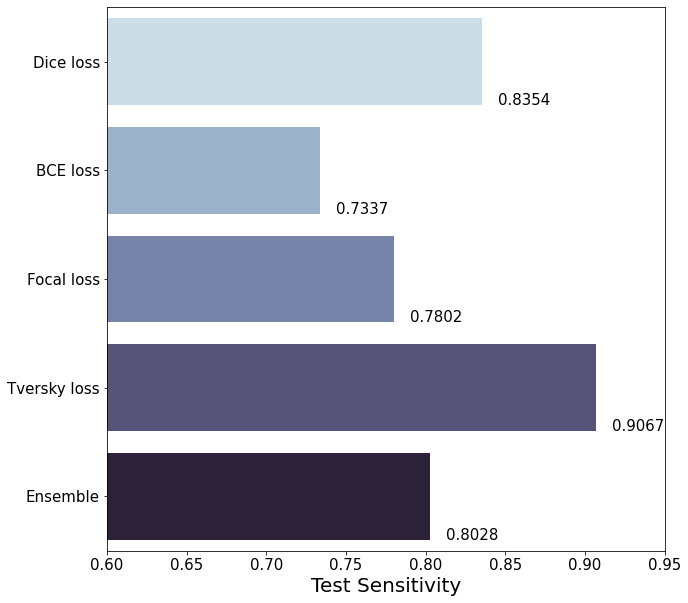
\includegraphics[scale=0.2]{original_data_sensitivity.png}
  \caption{Sensitivity from models trained on original dataset}
  \label{original_data_sensitivity}
\end{figure}
\begin{figure}[tp]
  \centering
  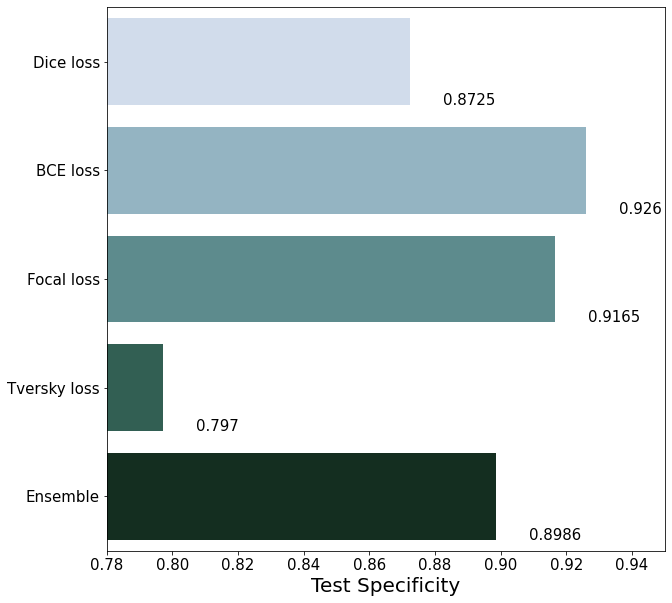
\includegraphics[scale=0.2]{original_data_specificity.png}
  \caption{Specificity from models trained on original dataset}
  \label{original_data_specificity}
\end{figure}
This is likely due to the Tversky function having strong weighting applied to
increase the significance of false negatives over false positives.  The
compromise to achieve such a high sensitivity score for the Tversky using
model can be seen in its fairly low specificity score.  The ensemble and other
base models utilizing different loss functions observed an opposite balance
with higher specificity than sensitivity which is to be expected when there are
more negative samples present.

\subsection{Training Against Undersampled Dataset}
Where the ensemble model really shined was in the model training
runs which used a higher class imbalance with a 10:1 negative to positive class
ratio.  Although balanced accuracy suggests that the ensemble model only has a
slight advantage over the other models, the sensitivity and specificity once
again help provide a complete picture.
\begin{figure}[tp]
  \centering
  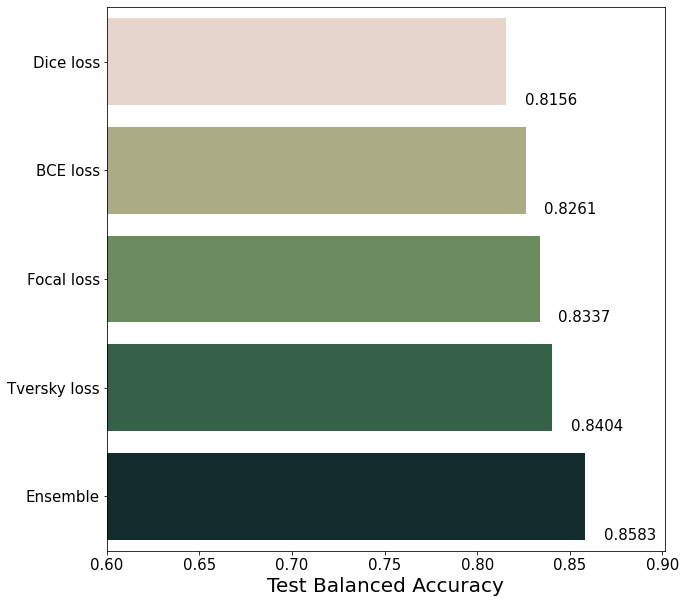
\includegraphics[scale=0.2]{undersampled_data_balanced_accuracy.png}
  \caption{Balanced Accuracy from models trained on dataset with reduced positive samples}
  \label{undersampled_data_balanced_accuracy}
\end{figure}
In this test run, all base models utilizing specialized loss functions had
substantially higher specificities than sensitivities.
\begin{figure}[tp]
  \centering
  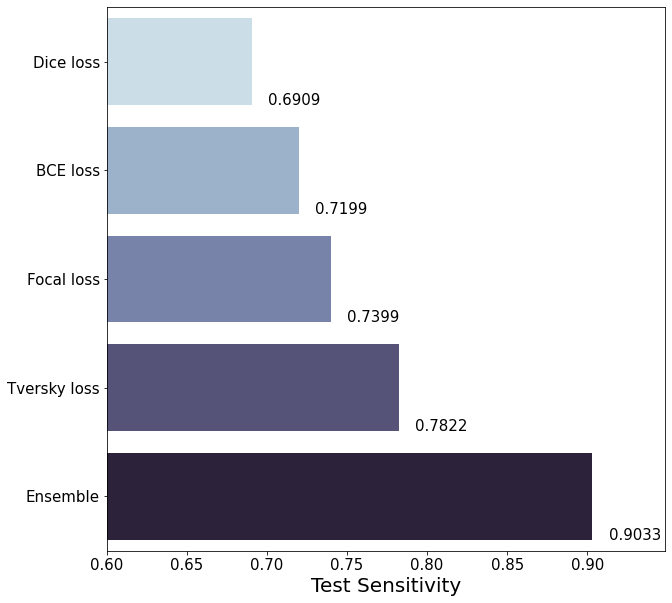
\includegraphics[scale=0.2]{undersampled_data_sensitivity.png}
  \caption{Sensitivity from models trained on dataset with reduced positive samples}
  \label{undersampled_data_sensitivity}
\end{figure}
\begin{figure}[tp]
  \centering
  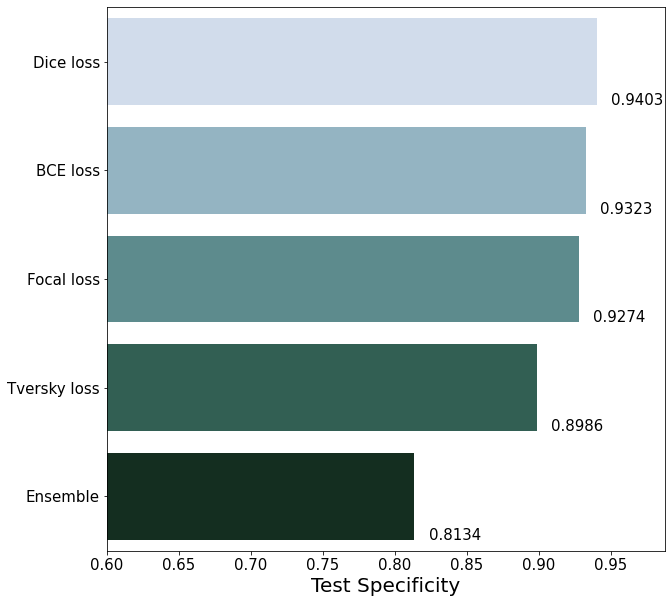
\includegraphics[scale=0.2]{undersampled_data_specificity.png}
  \caption{Specificity from models trained on dataset with reduced positive samples}
  \label{undersampled_data_specificity}
\end{figure}
As mentioned before, this is the expected result when training data with such a
large imbalance.  Where the base models struggled to detect positive classes,
the ensemble model prevailed with a sensitivity marginally higher than the
other models.  With the ensemble model using a number of base models equal to
the amount of equally sized partitions in the negative class with size
proportional to the positive class, this training run involved an ensemble
model with 10 individually trained base models as opposed to the previous
training run which only used 3.  This suggests that the ensemble model should
continue to perform better than more traditional models as the disparity
between classes grows and the number of individually trained base models
increases.


\section{Conclusion}
In summary, each of the models in the ensemble sees a different part of the
majority class and the same part of the minority class; the model’s predictions
are then averaged so they form one whole model that has seen the entire
dataset. Due to this our method eliminates the wasting of data caused by
under-sampling the majority class since all the samples are still used. It also
eliminates the overfitting caused by oversampling the minority class since each
model only sees each of the minority class samples once.
\\ \indent In the graphs for the original dataset that was 72\% cancer negative
and 28\% cancer positive our model had very similar balanced accuracy to the
best performing weighted losses only having 0.32\% less than the best balanced
accuracy. This is not surprising as the weighted losses work decently well when
the dataset imbalance is not too extreme. Where our model becomes the clear
winner is when the skew between the positive and negative classes becomes
larger with the dataset being 90\% cancer negative and only 10 \% cancer
positive. Here our models balanced accuracy becomes between 1.8\%-4\% better than
the other models. The best part is when you look at our models sensitivity
which is a very important metric for cancer classification as it makes sure we
have captured all the positive cases since the consequences of classifying
someone not to have cancer when they do is very serious. Here our model
performs between 12-21\% better than the other models. This is excellent as it
shows our ensemble balancing method performs better as the skew gets larger and
with larger datasets usually having even bigger skews where the cancer positive
class can sometimes only be 1\% of the dataset we expect the performance gap to
increase.


\bibliography{progress_report_ref}

\section{Code Submission}
All code for this project can be found in the
\underline{
\href{https://github.com/svecile/Breast-Histopathology-Classification}
  {group's github repository}.}

\end{document}
